\section{Introduktion}\label{sec:introduktion}
	Dette projekt er støttet af NNF (Novo Nordisk Fonden) og formålet med det generelle projekt er at lade elever prøve at arbejde som forskere. Dertil har eleverne udviklet en station som skulle indsamle data. Dataet bliver behandlet af lærere på Rybners HTX, som vil blive brugt i undervisningsforløb til folkeskoler og arbejdsopgaver til gymnasiet. Denne arbejdsgruppe arbejder med at opbygge en datalogger, som skal kunne indsamle diverse data via forskellige sensorer. Dette dokument beskriver, hvordan hver sensor er sat op, hvilke kodevalg der er blevet gjort, og hvordan programmet bliver kørt igennem. Hvert kapitel i dokumentet, efter Kode og Flowcharts, angiver en sensor og hvordan den er sat op. 
	\subsection{Forbindelser i Arduinoen}
		Her er et overblik over hvilke porte som er i brug på Arduino Mega'en. Der er blevet brugt et program kaldet Fritzing til at visualisere, hvordan de forskellige sensorer og moduler er forbundet til Arduinoen (Se kapitel \ref{sec:VisuelDatalogger}). På grund af det høje antal af moduler og kabler er der oplyst herunder for hvert modul, hvor og hvordan det enkelte modul er forbundet til Arduinoen. (Det vil også stå inde under hver moduls sektion)\\ [7pt]
		\begin{minipage}{0.49\textwidth}
			RTC (Real Time Clock):
			\begin{itemize}
				\item 5V - 5V
				\item GND - GND
				\item SCL - Port 21 (SCL)
				\item SDA - Port 20 (SDA)
			\end{itemize}
			SD Card Module:
			\begin{itemize}
				\item +5 - 5V
				\item +3.3 - 3.3V
				\item GND - GND
				\item CS - Port 53 (SS)
				\item MOSI - Port 51 (MOSI)
				\item SCK - Port 52 (SCK)
				\item MISO - Port 50 (MISO)
			\end{itemize}
		\end{minipage}
		\hfill
		\begin{minipage}{0.49\textwidth}
			Digital Temperatur Sensor (DS18B20):
			\begin{itemize}
				\item Rød ledning - 5V
				\item Sort ledning - GND
				\item Gul ledning - 5V $\to$ 1K$\Omega$ resistor $\to$ Port 22
			\end{itemize}
			pH Sensor:
			\begin{itemize}
				\item V+ - 5V
				\item G - GND
				\item PO - A0
				\item TO - A1
			\end{itemize}
		\end{minipage}
		\newpage
		\begin{minipage}{0.49\textwidth}
			UV Sensor (VEML6075):
			\begin{itemize}
				\item 3Vo - 3.3V
				\item GND - GND
				\item SCL - Port 21 (SCL)
				\item SDA - Port 20 (SDA)
			\end{itemize}
			Tryksensor (MLP3115A2):
			\begin{itemize}
				\item 3Vo - 3.3V
				\item GND - GND
				\item SCL - Port 21 (SCL)
				\item SDA - Port 20 (SDA)
			\end{itemize}
		\end{minipage}
		\hfill
		\begin{minipage}{0.49\textwidth}
			MQ2 Gas Sensor:
			\begin{itemize}
				\item VCC - 5V
				\item GND - GND
				\item NC - N/A
				\item SIG(AO) - A2
			\end{itemize}
		\end{minipage}
		
	\newpage
	\subsubsection{Opbygning af datalogger visualiseret}\label{sec:VisuelDatalogger}
		\begin{figure}[h!]
			\centering
			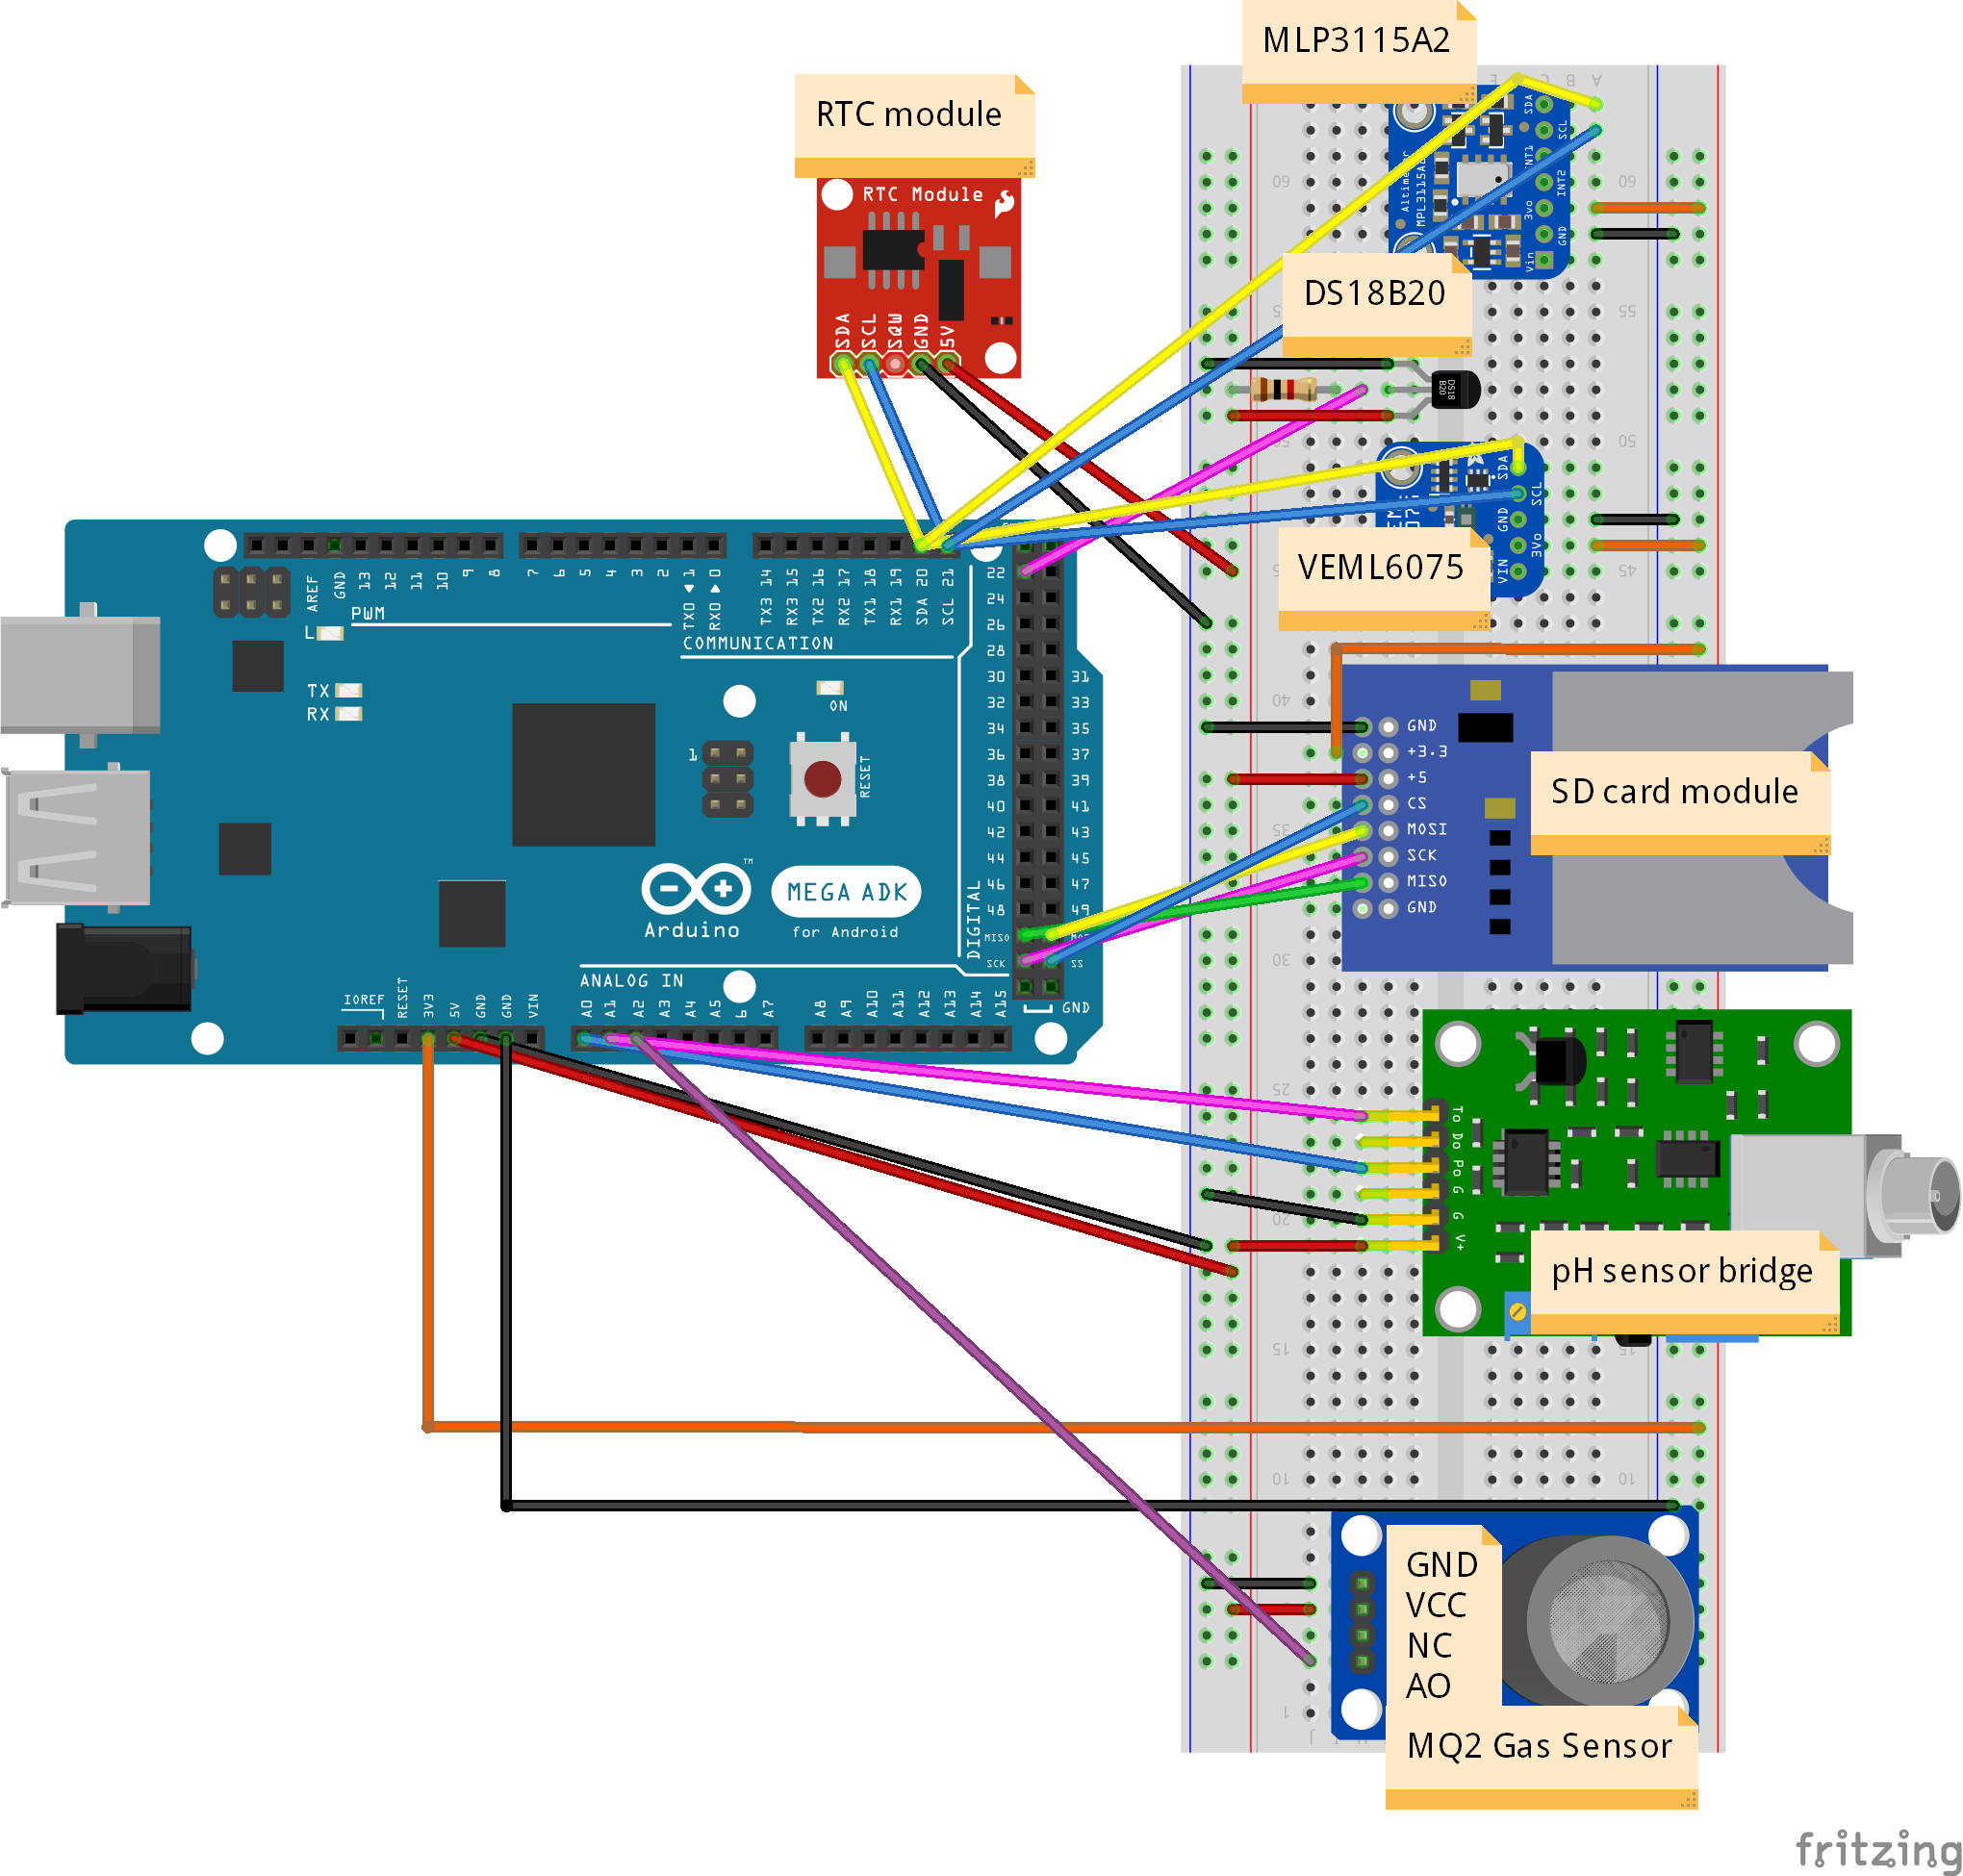
\includegraphics[width=\textwidth]{Figures/Diagram_v3.png}
			\caption{Opstillingen af nuværende datalogger lavet i Fritzing m. Arduino og moduler} \label{fig:Opstilling}
		\end{figure}